%! Author = joels
%! Date = 05/01/2021

\section{Berechtigungen, Persistenz und Hardwarezugriff}
\subsection{Berechtigungen}
\subsubsection{Grundlagen}
Apps dürfen nur Aktionen ausführen, die andere Dienste nicht negativ beeinflussen (Sandbox). Vor riskanten Operationen müssen Berechtigungen eingeholt werden:
\begin{itemize}[topsep=0pt, leftmargin=4mm]
    \setlength\itemsep{-0.3em}
    \item Zugriff auf System APIs (Internet, WiFi, Bluetooth, etc. )
    \item Zugriff auf sensitive Daten (Telefonanruf, Kontaktliste, Kalender, etc.)
    \item Zugriff auf bestimmte Hardware (Kamera, Lokalisierung, etc.)
\end{itemize}
Es gibt zwei Arten von Berechtigungen:\\
\textcolor{blue}{Normal:} Werden durch das System erteilt.\\
\textcolor{blue}{Gefährlich:} Werden durch den Benutzer erteilt.\\
\textbf{\textcolor{blue}{Berechtigungen erteilen:}}\\
Bis API 22 (Android 5.1.1): Während Installation der App. Kein selektives Ablehnen möglich.\\
Ab API 23 (Android 6.0): Während Nutzung der App. Selektives Ablehnen möglich.\\
Ab API 30 (Android 11.0): Weiterhin während Nutzung. Dialog ergänzt um "Einmalig"-Option\\
\textbf{\textcolor{blue}{Berechtigungen verwalten:}}\\
Berechtigungen können vom Benutzer zurückgezogen werden. Seit API 30 können Berechtigungen vom System zurückgesetzt werden. \textbf{Darum Empfehlung:} Kein Flag zum Abfragen der Berechtigung setzten in der App, sondern immer Zugriff überprüfen. Sonst wird Berechtigung vom System entzogen aber Flag im Code ist gesetzt. SecurityException: Wenn keine Berechtigung, gut zum Debuggen wenn App abstürzt.\\
\textbf{\textcolor{blue}{Best Practices:}}
\begin{itemize}[topsep=0pt, leftmargin=4mm]
    \setlength\itemsep{-0.3em}
    \item Nur anfordern, was auch benötigt wird
    \item Im Kontext der Verwendung anfordern
    \item Transparente Erklärungen
    \item Abbruch ermöglichen
    \item Verweigerung berücksichtigen
\end{itemize}
\subsubsection{Berechtigungen XML/Code}
\textbf{\textcolor{blue}{Manifest:}}
Benötigte Berechtigungen müssen im Manifest deklariert werden. Knoten \textcolor{blue}{$<$uses-permission$>$}\\
Hinweise auf benötigte Features für Filterung im Google Play Store. Knoten \textcolor{blue}{$<$uses-feature$>$} $\rightarrow$ Ist optional, aber empfohlen
\begin{lstlisting}
// AndroidManifest.xml
<?xml version="1.0" encoding="utf-8"?>
<manifest>
<!-- Berechtigungen -->
<uses-permission
    android:name="android.permission.CALL_PHONE"/>
<uses-permission
    android:name="android.permission.CAMERA"/>
<uses-permission
    android:name="android.permission.WRITE_EXTERNAL_STORAGE"
    android:maxSdkVersion="28" />
<!-- Feature-Hinweise -->
<uses-feature
    android:name="android.hardware.location" />
<uses-feature
    android:name="android.hardware.camera"
    android:required="true" />
<uses-feature
    android:name="android.hardware.bluetooth"
    android:required="false" />
</manifest>
\end{lstlisting}
\textbf{\textcolor{blue}{Anforderung im Code:}}
\begin{lstlisting}
// MainActivity.java
private static final int CALLBACK_CODE = 1;
String permission = Manifest.permission.CALL_PHONE;
// Aktuellen Status prüfen (AndroidX)
int status = ContextCompat.checkSelfPermission(
    this,
    permission);
if (status != PackageManager.PERMISSION_GRANTED) {
    if (shouldShowRequestPermissionRationale(permission)) {
        // Erklärung für Benutzer anzeigen (Wozu nötig?)
    }
    // Berechtigung beim Benutzer anfordern
    requestPermissions(
        new String[]{ permission },
        CALLBACK_CODE);
}

@Override
public void onRequestPermissionsResult(
    int requestCode, String[] permissions, int[] results) {
    if (requestCode != CALLBACK_CODE)
        return;
    if (results.length == 0)
        return; // Anfrage abgebrochen
    if (results[0] == PackageManager.PERMISSION_GRANTED) {
        // Berechtigung erteilt
    } else {
        // Berechtigung verweigert
    }
}
\end{lstlisting}
\textbf{\textcolor{blue}{Hinweis:}}\\
falls der benutzer \dq Nicht mehr fragen\dq auswählt, werden keine Dialoge mehr angezeigt. Ab API 30 gelten wiederholte Ablehnungen automatisch als \dq Nicht mehr fragen\dq.

\subsection{Persistenz}
\subsubsection{Speicherarten}
\textbf{\textcolor{blue}{Interner Speicher:}}
\begin{itemize}[topsep=0pt, leftmargin=4mm]
    \setlength\itemsep{-0.3em}
    \item Stets verfügbar
    \item Geschützter Speicherbereich pro App
    \item Speicherplatz begrenzt
    \item Für app-interne Daten
\end{itemize}
\textbf{\textcolor{blue}{Externer Speicher:}}
\begin{itemize}[topsep=0pt, leftmargin=4mm]
    \setlength\itemsep{-0.3em}
    \item Nicht immer verfügbar
    \item Oft ein Wechseldatenträger
    \item Emulation durch Android möglich
    \item Speicherplatz begrenzt (aber meist grösser)
    \item Primär für geteilte Daten
\end{itemize}
Bis API 28 konnte eine App auf beliebige Medien im externen Speicher zugreifen, brauchte dazu aber Berechtigungen.\\
Seit API 29 kann eine App eigene Medien im externen Speicher ohne Berechtigungen lesen und
schreiben. Der Zugriff auf Medien von fremden Apps ist nur noch lesend möglich und braucht eine Berechtigung.\\
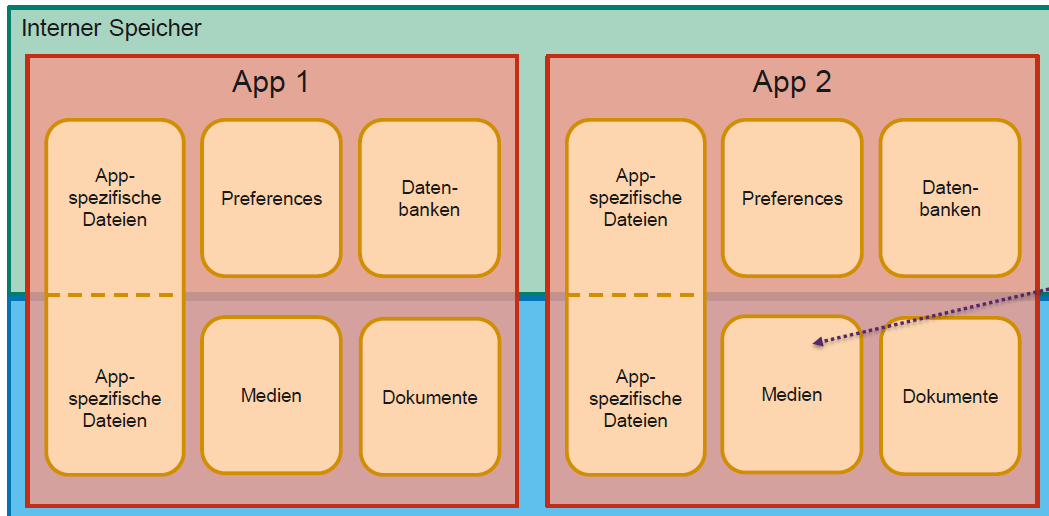
\includegraphics{persistenz.png}
\subsubsection{App-spezifische Dateien}
\begin{itemize}[topsep=0pt, leftmargin=4mm]
    \setlength\itemsep{-0.3em}
    \item Eigene, proprietäre Datenformate
    \item Interner oder externer Speicher
    \item Bei Deinstallation der App gelöscht
    \item Geschützt vor fremdem Zugriff
    \item Keine Berechtigungen nötig (seit API 19)
    \item Zugriff via File-API und Context
    \begin{itemize}[topsep=0pt, leftmargin=4mm]
        \setlength\itemsep{-0.3em}
        \item Context.getFilesDir()
        \item Context.getCacheDir()
        \item Context.getExternalFilesDir()
        \item Context.getExternalCacheDir()
    \end{itemize}
\end{itemize}
\begin{lstlisting}
// Schreiben
File folder = getFilesDir();
File file = new File(folder, "my_file.txt");
String input = "MGE Beispiel";
FileOutputStream outputStream = new FileOutputStream(file);
outputStream.write(input.getBytes());
outputStream.close();

// Dateien anzeigen
for(File fileInFolder : folder.listFiles()) {
    Log.d("MGE.V05", "File: " + fileInFolder.getName());
}

// Lesen
int length = (int) file.length();
byte[] bytes = new byte[length];
FileInputStream inputStream = new FileInputStream(file);
inputStream.read(bytes);
inputStream.close();
String output = new String(bytes);
\end{lstlisting}
\subsubsection{Preferences}
\begin{itemize}[topsep=0pt, leftmargin=4mm]
    \setlength\itemsep{-0.3em}
    \item Key-Value-Paare
    \item Interner Speicher
    \item Bei Deinstallation der App gelöscht
    \item Keine Berechtigungen nötig
    \item Zugriff via SharedPreferences-Objekte
    \begin{itemize}[topsep=0pt, leftmargin=4mm]
        \setlength\itemsep{-0.3em}
        \item Context.getSharedPreferences(name, mode)
        \item Activity.getPreferences(mode)
    \end{itemize}
    \item AndroidX: EncryptedSharedPreferences
\end{itemize}
\begin{lstlisting}
String file = "ch.ost.rj.mge.v05.myapp.preferences";
String key1 = "my.key.1";
String key2 = "my.key.2";
String key3 = "my.key.3";
int mode = Context.MODE_PRIVATE;

// Objekt abholen
SharedPreferences preferences;
preferences = getSharedPreferences(file, mode);

// Schreiben
SharedPreferences.Editor editor = preferences.edit();
editor.putString(key1, "MGE Beispiel");
editor.putBoolean(key2, true);
editor.putInt(key3, 42);
editor.commit();

// Lesen
String value1 = preferences.getString(key1, "default");
boolean value2 = preferences.getBoolean(key2, false);
int value3 = preferences.getBoolean(key3, 0);
\end{lstlisting}
\subsubsection{Content Providers}
\begin{itemize}[topsep=0pt, leftmargin=4mm]
    \setlength\itemsep{-0.3em}
    \item Datenquelle für andere Apps
    \item Client-Server Modell
    \begin{itemize}[topsep=0pt, leftmargin=4mm]
        \setlength\itemsep{-0.3em}
        \item Client: Content Resolver
        \item Server: Content Provider
    \end{itemize}
    \item SQL-ähnliche, standardisierte Schnittstelle
    \item Android enthält diverse Provider: Kalender, Kontakte, Medien, Dokumente, Wörterbuch
\end{itemize}
\subsubsection{Content Resolvers}
\begin{itemize}[topsep=0pt, leftmargin=4mm]
    \setlength\itemsep{-0.3em}
    \item Zugriff auf Provider via ContentResolver
    \item Bietet Methoden für CRUD-Operationen
    \item Iteration über Ergebnisse via Cursor
    \item Berechtigung nötig für Zugriff auf Daten
\end{itemize}
\begin{lstlisting}
Cursor cursor = getContentResolver().query(
    uri,
    projection,
    selection,
    selectionArgs,
    sortOrder
);
\end{lstlisting}
\subsubsection{Medien}
\begin{itemize}[topsep=0pt, leftmargin=4mm]
    \setlength\itemsep{-0.3em}
    \item Teilbare Bilder, Videos und Musik
    \item Externer Speicher
    \item Bleiben bei Deinstallation der App erhalten
    \item Berechtigungen
    \begin{itemize}[topsep=0pt, leftmargin=4mm]
        \setlength\itemsep{-0.3em}
        \item bis API 28: für jegliches Lesen oder Schreiben
        \item ab API 29: nur für das Lesen fremder Dateien
    \end{itemize}
    Zugriff via MediaStore (Content Provider)
\end{itemize}
\begin{lstlisting}
// Auslesen von Bildern sortiert nach Einfügedatum
String[] projection = new String[] {
    MediaStore.Images.Media.TITLE,
    MediaStore.Images.Media.DATE_ADDED
};
String order = MediaStore.Images.Media.DATE_ADDED + " DESC";
Cursor cursor = getContentResolver().query(
    MediaStore.Images.Media.EXTERNAL_CONTENT_URI,
    projection, // projection
    null, // selection
    null, // selectionArgs
    order // sortOrder
);
int ct = cursor.getColumnIndex(MediaStore.Images.Media.TITLE);
int cd = cursor.getColumnIndex(MediaStore.Images.Media.DATE_ADDED);
while (cursor.moveToNext()) {
    String title = cursor.getString(ct);
    long added = cursor.getLong(cd);
    // ... hier die Werte verwenden ...
}
cursor.close();
\end{lstlisting}
\subsubsection{Dokumente}
\begin{itemize}[topsep=0pt, leftmargin=4mm]
    \setlength\itemsep{-0.3em}
    \item Teilbare Dokumente wie PDF, ZIP, etc.
    \item Externer Speicher
    \item Bleiben bei Deinstallation der App erhalten
    \item Keine Berechtigungen nötig
    \item Zugriff via Storage Access Framework (Kombination aus Intents \& Content Provider)
    \item Auswahl von Dokumenten via "Picker"
\end{itemize}
\subsubsection{Datenbanken}
\begin{itemize}[topsep=0pt, leftmargin=4mm]
    \setlength\itemsep{-0.3em}
    \item Strukturierte Daten
    \item Interner Speicher
    \item Bei Deinstallation der App gelöscht
    \item Keine Berechtigungen nötig
    \item Zugriff auf zwei Arten: SQLite API, Room aus AndroidX/Jetpack (Wrapper um SQLite)
\end{itemize}
\subsubsection{Datenbanken – Room}
\begin{itemize}[topsep=0pt, leftmargin=4mm]
    \setlength\itemsep{-0.3em}
    \item Abstraktionsschicht über SQLite
    \item ORM (Object Relational Mapping)
    \begin{itemize}[topsep=0pt, leftmargin=4mm]
        \setlength\itemsep{-0.3em}
        \item Abbildung von DB-Tabellen auf Java-Klassen
        \item Basiert auf Java-Annotations
    \end{itemize}
    \item Vorteile
    \begin{itemize}[topsep=0pt, leftmargin=4mm]
        \setlength\itemsep{-0.3em}
        \item Weniger Code nötig (z.B. Mapping)
        \item Überprüfung von Queries zur Compile-Zeit
        \item Kompatibilität mit Jetpack-Komponenten
    \end{itemize}
\end{itemize}
\begin{lstlisting}
// Entry.java
@Entity
public class Entry {
    @PrimaryKey(autoGenerate = true)
    public int id;

    @ColumnInfo
    public String content;
}

// EntryDao.java
@Dao
public interface EntryDao {
    @Query("SELECT * FROM entry")
    List<Entry> getEntries();

    @Insert
    void insert(Entry entry);

    @Delete
    void delete(Entry entry);
}

// EntryDatabase.java
@Database(entities = {Entry.class}, version = 1)
public abstract class EntryDatabase extends RoomDatabase {
    public abstract EntryDao entryDao();
}

// MainActivity.java
// Erzeugung DB-Objekt
EntryDatabase db = Room.databaseBuilder(this, EntryDatabase.class, "room.db")
    .build();
EntryDao dao = db.entryDao();

// Daten einfügen
Entry entry = new Entry();
entry.content = "MGE Vorlesung";
dao.insert(entry);

// Daten auslesen
List<Entry> entries = dao.getEntries();
for (Entry entry : entries) {
    Log.d(null, + entry.id + " | " + entry.content);
}

// Aufräumen
db.close();
\end{lstlisting}

\subsection{Hardwarezugriff}
\subsubsection{Grundlagen}
Smartphones besitzen diverse \textcolor{blue}{Aktoren} \& \textcolor{blue}{Sensoren}. z.B: Display, Lautsprecher, Vibration, Kamera, Beschleunigung, Licht, Lage.\\
\textbf{\textcolor{blue}{Sensor Framework:}}
\begin{itemize}[topsep=0pt, leftmargin=4mm]
    \setlength\itemsep{-0.3em}
    \item \textcolor{blue}{SensorManager} als Einstiegspunkt 
    \item \textcolor{blue}{Sensor} als Repräsentant für realen Sensor 
    \item \textcolor{blue}{SensorEvent} enthält Werte des Sensors 
    \item \textcolor{blue}{SensorEventListener}für Callbacks
\end{itemize}
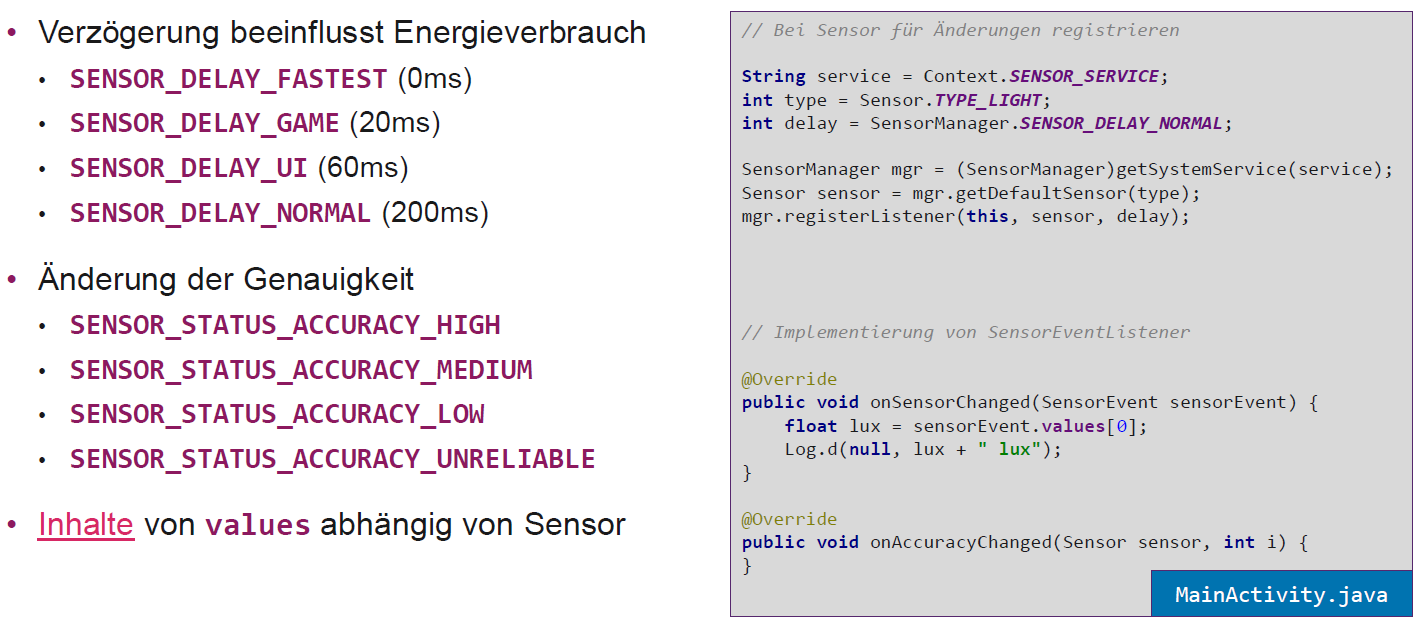
\includegraphics{sensor_framework.png}
\subsubsection{Vibration}
Verwendung der Klasse \textcolor{blue}{Vibrator}. Berechtigung nötig (VIBRATE)\\
Ab API26: \textcolor{blue}{createOneShot()} (erlaubt Stärke der Vibration) und \textcolor{blue}{createWaveform()} (für komplexe Muster).\\
Ab API29: \textcolor{blue}{createPredefined()} für Standard-Effekte.
\begin{lstlisting}
String service = Context.VIBRATOR_SERVICE;
int maxAmplitude = 255;
Vibrator vibrator = (Vibrator) getSystemService(service);
// Ab API 1
vibrator.vibrate(500);
Vibrator.cancel();
// Ab API 26
long[] durs = new long[]{ 500, 500, 500, 500, 500 };
int[] amps = new int[]{ 50, 100, 150, 200, 255 };
VibrationEffect effect;
effect = VibrationEffect.createOneShot(500, 255);
effect = VibrationEffect.createWaveform(durs, amps, -1);
vibrator.vibrate(effect);
// Ab API 29
int effectId = VibrationEffect.EFFECT_DOUBLE_CLICK;
effect = VibrationEffect.createPredefined(effectId);
vibrator.vibrate(effect);
\end{lstlisting}
\subsubsection{Connectivity Internet}
Über Klasse \textcolor{blue}{ConnectivityManager}. Üblich sind zwei Kanäle (Wifi \& Mobile). Android nutzt automatisch besten Kanal (Höhere Geschwindigkeit, Bessere Signalqualität, Kein Roaming). Berechtigung nötig: ACCESS\_NETWORK\_STATE.
\begin{lstlisting}
String service = Context.CONNECTIVITY_SERVICE;
ConnectivityManager manager;
manager = (ConnectivityManager) getSystemService(service);

// Aktive Verbindung prüfen
NetworkInfo activeNetwork = manager.getActiveNetworkInfo();
if (activeNetwork != null) {
    int type = activeNetwork.getType();
    Log.d(null, "Active connection: " + type);
}
// Verbindungen prüfen
for (Network network : manager.getAllNetworks()) {
    NetworkInfo info = manager.getNetworkInfo(network);
    boolean state = info.isConnected();
    if (info.getType() == ConnectivityManager.TYPE_WIFI) {
        Log.d(null, "WiFi is connected: " + state);
    }
    if (info.getType() == ConnectivityManager.TYPE_MOBILE) {
        Log.d(null, "Mobile is connected: " + state);
    }
}
\end{lstlisting}